%-----------------------------------------------------------------------
%
\section{Examples}
\label{example}
%
%-----------------------------------------------------------------------

This section presents several examples to illustrate how the
implementation of the $\overline{\gamma}_{\alpha}-autotuning$
improves the performance of the closed-loop system respect to the
both operation modes.

In all the examples it is supposed that the process output can
vary in the 0 to 100\% normalized range and that in the normal
operation point, the controlled variable has a value close to
70\%.

\subsection{Example 1}

Let us to consider the system (\ref{system_example}), shown before
as a \emph{Motivation Example}.

Table \ref{PID_parameters} shows the PID controller parameters for
the system (\ref{system_example}) using the
\cite{zhuangAthertonIEE1993} method and the proposed
$\overline{\gamma}_{\alpha}-autotuning$ with $\alpha=\{0.25, 0.50,
0.75\}$. Moreover, the corresponding system outputs responses to a
20\% set-point change followed by a -20\% load-disturbance change,
are shown in Fig. \ref{y_out} for the following tuning methods:
set-point, load-disturbance and
$\overline{\gamma}_{\alpha}-autotuning$ with its three possible
scenarios. The control signal is not shown for the sake of
brevity, however it can be easily guessed that it would be
smoother when the value of $\alpha$ is lower (see Example 3).

\begin{table}[h!]
\begin{center}
\caption{Example 1 - PID Controller Parameters}
\begin{tabular}{c|ccc}
\hline \textbf{tuning}               &$K_p$ &$T_i$ &$T_d$\\ \hline
$set-point(sp)$                               &1.657  &1.694  &0.513 \\
$load-disturbance(ld)$                        &2.418  &1.007  &0.559 \\
\hline
$\overline{\gamma}_{\alpha=0.25}-autotuning$  &1.791  &1.378  &0.520 \\
$\overline{\gamma}_{\alpha=0.50}-autotuning$  &1.949  &1.234  &0.527 \\
$\overline{\gamma}_{\alpha=0.75}-autotuning$  &2.016  &1.177  &0.531 \\
\hline
\end{tabular}
\label{PID_parameters}
\end{center}
\end{table}

\begin{figure}[htb!]
    \begin{center}
        \includegraphics[width=0.8\linewidth]{youtp0.eps}
        %\includegraphics[width=0.8\linewidth]{y_outp.eps}
        \caption{Example 1 - Process output for the control system operating in both servo and regulation modes}
        \label{y_out}
    \end{center}
\end{figure}

It can be seen that the proposed
$\overline{\gamma}_{\alpha}-autotuning$ gives lower performance
than the optimum settings when the system operates in the same way
as it was tuned. However, higher performance can be obtained for
the whole system operation (regulatory-control and servo-control),
when an \emph{intermediate} controller is used.

Table \ref{values_PD} shows the Performance Degradation values
calculated from (\ref{PD_gamma_servo}) to (\ref{global_pd}) and
also the $\mathit{WPD}$ index (\ref{alpha_pd}) for each tuning.
The below side of the table presents the improvement in percentage
that can be achieved with each one of the
$\overline{\gamma}_{\alpha}-autotuning$ respect to the extreme
tunings (set-point and load-disturbance).

\begin{table}[h!]
\begin{center}
\caption{Example 1 - $\mathit{PD}$ and $\mathit{WPD}$ values for
the system (\ref{system_example}) and the improvement obtained
with $\overline{\gamma}_{\alpha}-autotuning$}
\begin{tabular}{c|cc|ccc}
\hline \textbf{tuning}       &$PD_{sp}$  &$PD_{ld}$ &$WPD_{\alpha=0.25}$ &$WPD_{\alpha=0.50}$ &$WPD_{\alpha=0.75}$\\
\hline
$set-point(sp)$                               &-          &0.3951 &0.0988 &0.1976 &0.2964\\
$load-disturbance(ld)$                        &0.9496     &-      &0.7123 &0.4748 &0.2374\\
%$\gamma-autotuning$                           &0.1129     &0.0534 &0.0980 & &\\
$\overline{\gamma}_{\alpha=0.25}-autotuning$  &0.0336     &0.1662 &0.0668 &- &-\\
$\overline{\gamma}_{\alpha=0.50}-autotuning$  &0.1088     &0.0376 &- &0.0732 &-\\
$\overline{\gamma}_{\alpha=0.75}-autotuning$  &0.1578     &0.0009 &- &- &0.0401\\
\hline \hline
improvement in \% of                          &            &            & & &\\
\hline
$\overline{\gamma}_{\alpha=0.25}-autotuning$  &96.46\%(ld) &57.93\%(sp) &32.39\%(sp) &- &-\\
                                              &            &            &90.62\%(ld) &- &-\\
$\overline{\gamma}_{\alpha=0.50}-autotuning$  &88.54\%(ld) &90.49\%(sp) &- &62.95\%(sp) &-\\
                                              &            &            &- &85.58\%(ld) &-\\
$\overline{\gamma}_{\alpha=0.75}-autotuning$  &83.38\%(ld) &99.77\%(sp) &- &- &86.47\%(sp)\\
                                              &            &            &- &- &83.11\%(ld)\\
(respect to)                                  &            &            & & &\\
\hline
\end{tabular}
\label{values_PD}
\end{center}
\end{table}

All the values confirm the fact that, in global terms, when both
operating modes could appear and taking into account the
importance that the control-loop is operating as servo or
regulation mode, the proposed
$\overline{\gamma}_{\alpha}-autotuning$ is the best choice to tune
the PID controller in order to get less Performance Degradations.

\subsection{Example 2}

In order to add completeness to the comparison, a case-study
example is provided. We consider the isothermal Continuous Stirred
Tank Reactor (CSTR), as the one in Fig. \ref{CSTR}, where the
isothermal series/parallel Van de Vusse reaction \cite{VandeVusse,
VandeVusse2} is taking place. The reaction can be described by the
following scheme

\begin{align}
    A \overset{k_1}{\longrightarrow} B \overset{k_2}{\longrightarrow}C\\
    2 A \overset{k_3}{\longrightarrow} D \nonumber
\end{align}

\begin{figure}[htb!]
\centering
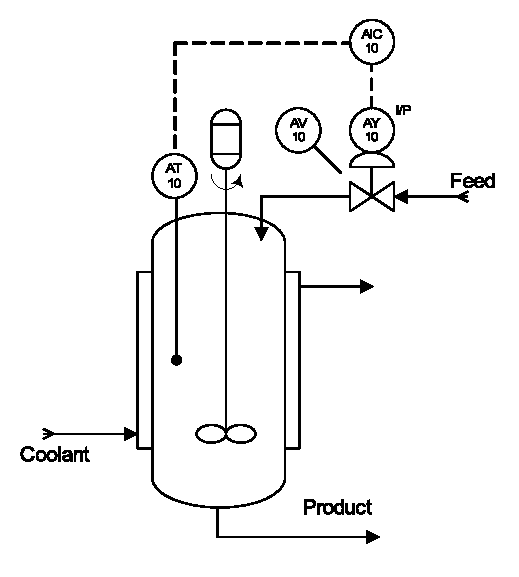
\includegraphics[width=0.5\linewidth]{Reactor02.eps}
\caption{Example 2 - CSTR System} \label{CSTR}
\end{figure}

Doing a mass balance, the system can be described by the following
model

\begin{align}
    \frac{dC_A(t)}{dt} & = \frac{F_r(t)}{V} \left[C_{Ai}-C_A(t)\right] - k_1 C_A(t) - k_3 C^2_A(t) \nonumber \\
    \frac{dC_B(t)}{dt} & = -\frac{F_r(t)}{V} C_B(t)+ k_1 C_A(t) - k_2 C_B(t)
    \label{system3}
\end{align}

\noindent where $F_r$ is the feed flow rate of product $A$, $V$ is
the reactor volume which is kept constant during the operation,
$C_A$ and $C_B$ are the reactant concentrations in the reactor,
and $k_i$ ($i=1,2,3$) are the reaction rate constants for the
three reactions.

In this case, the variables of interest are: the concentration of
$B$ in the reactor ($C_B$ as the controlled variable), the flow
through the reactor ($F_r$ as the manipulated variable), and the
concentration $C_{Ai}$ of $A$ in the feed flow (whose variation
can be considered as the disturbance). The kinetic parameters are
chosen to be $k_1 = 5/6 \ min^{-1}$, $k_2 = 5/3 \ min^{-1}$, and
$k_3 = 1/6 \ l \ mol^{-1} \ min^{-1}$. Also, is assumed that the
nominal concentration of $A$ in the feed ($C_{Ai}$) is $10 \ mol \
l^{-1}$ and the volume $V = 700 \ l$.

Using (\ref{system3}) and the parameters values, the
characterization of the steady-state for the process can be
obtained as it is shown in Fig.\ref{c_estatica}, for three
concentrations of $C_{Ai}$, where is easy to see the non-linearity
of the system.

\begin{figure}[htb!]
    \begin{center}
        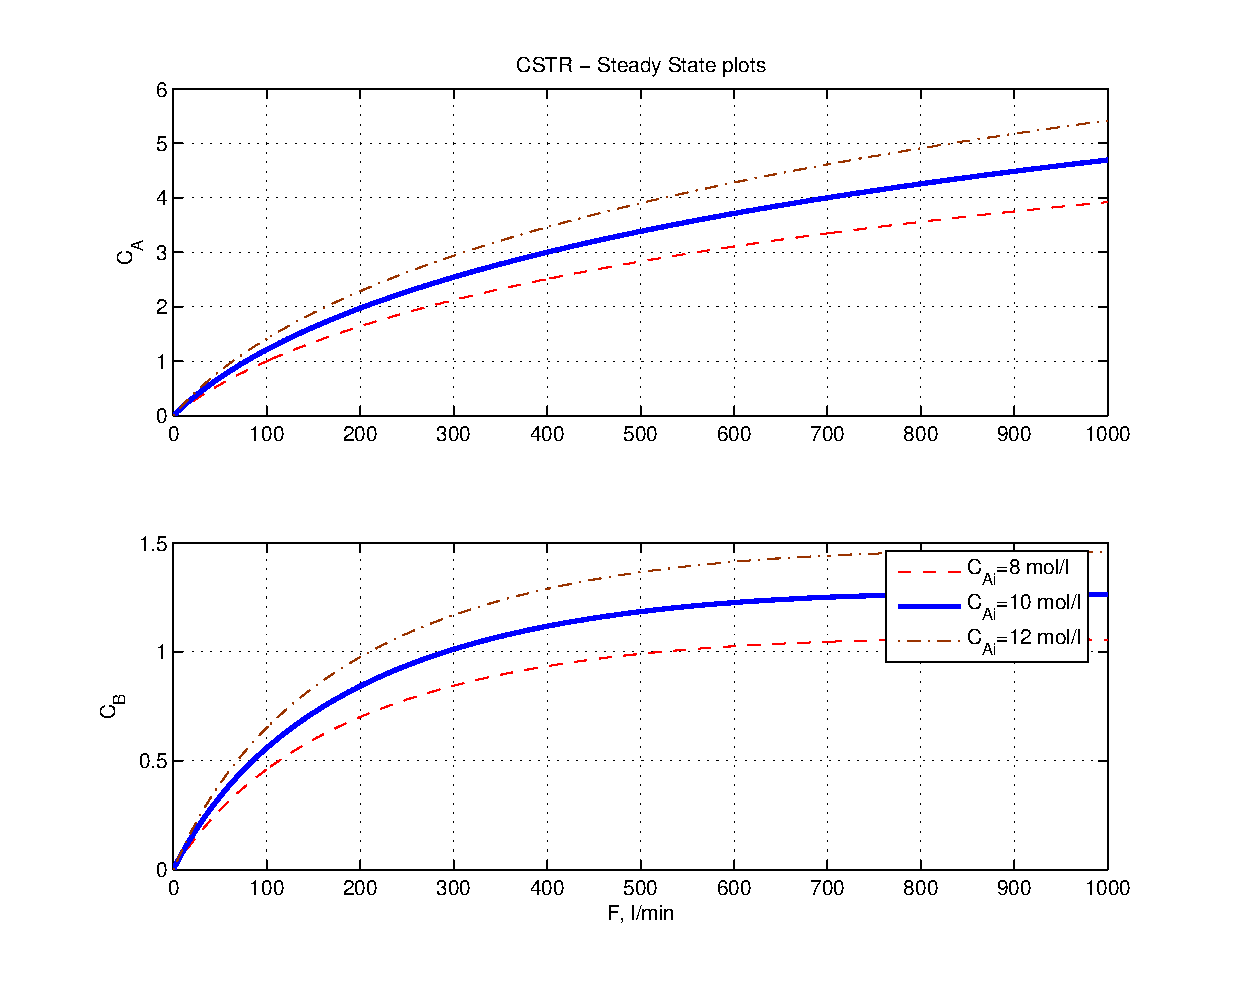
\includegraphics[width=0.7\linewidth]{c_estatica.eps}
        \caption{Example 2 - Steady-State characterization for the reactor}
        \label{c_estatica}
    \end{center}
\end{figure}

Initially, the system is at the steady-state (therefore the
operational point) with $C_{Ao} = 2.9175 \ mol \ l^{-1}$ and
$C_{Bo} = 1.10 \ mol \ l^{-1}$. From this, it can be selected the
measurement range for $C_B$ from $0$ to $1.5714 \ mol/l$ and the
capacity for the control valve with a maximum flow of $634.1719 \
l/min$ (variation range of the flow from $0$ to $634.1719 \
l/min$) \cite{arrietaETFA2008}. The signals ($y$, $u$, $r$) will
be in percentage ($0$ to $100\%$).

The sensor-transmitter element takes the form

\be
    y(t)_{\%} = \left(\frac{100}{1.5714}\right) C_B(t) \label{sensor}
\ee

\noindent and the control valve with a linear flow characteristic,

\be
    F_r(t) = \left(\frac{634.1719}{100}\right) u(t)_{\%} \label{actuator}
\ee

Fig.\ref{c_estatica2} shows the steady-state characterization,
taking into account elements represented by (\ref{sensor}) and
(\ref{actuator}). This is calling \emph{set
actuator-process-sensor} and from this is clearly that for the
selected steady-state, $r_o = 70 \%$ and $u_o = 60 \%$.

\begin{figure}[htb!]
    \begin{center}
        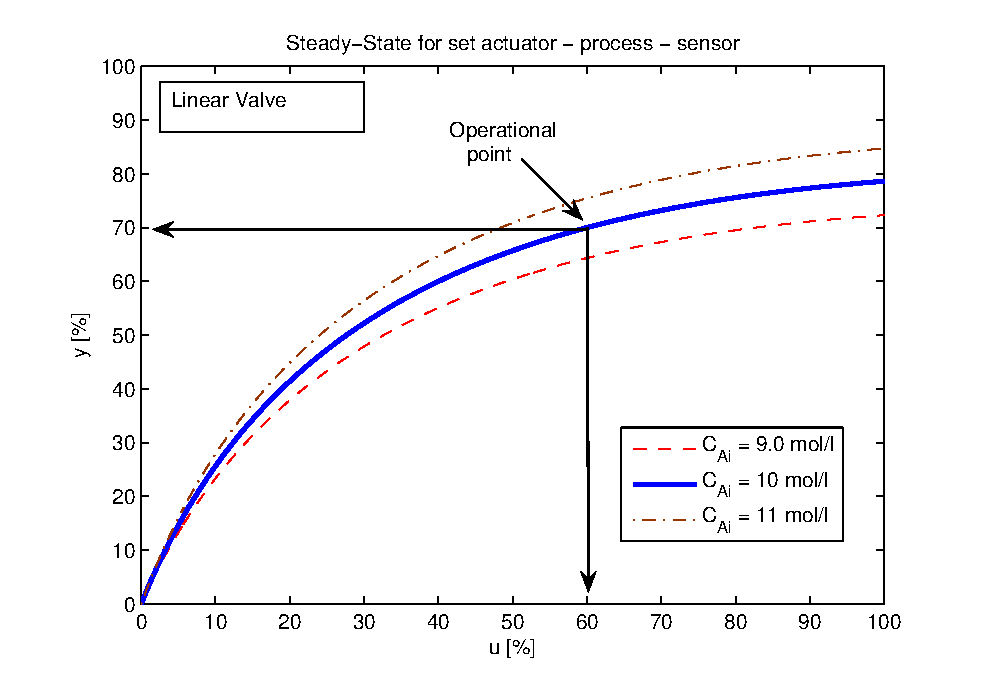
\includegraphics[width=0.7\linewidth]{c_estatica2.eps}
        \caption{Example 2 - Steady-State characterization for the set actuator-process-sensor}
        \label{c_estatica2}
    \end{center}
\end{figure}

It is assumed that changes in the set-point would be not bigger
than $10 \%$ and the possible disturbance in $C_{Ai}$, can variate
around $\pm 10 \%$. In Fig.\ref{process} can be seen the process
output (including the sensor and the control valve) and also the
FOPDT model for a step change in the process input ($y_u(t)$).

\begin{figure}[htb!]
    \begin{center}
        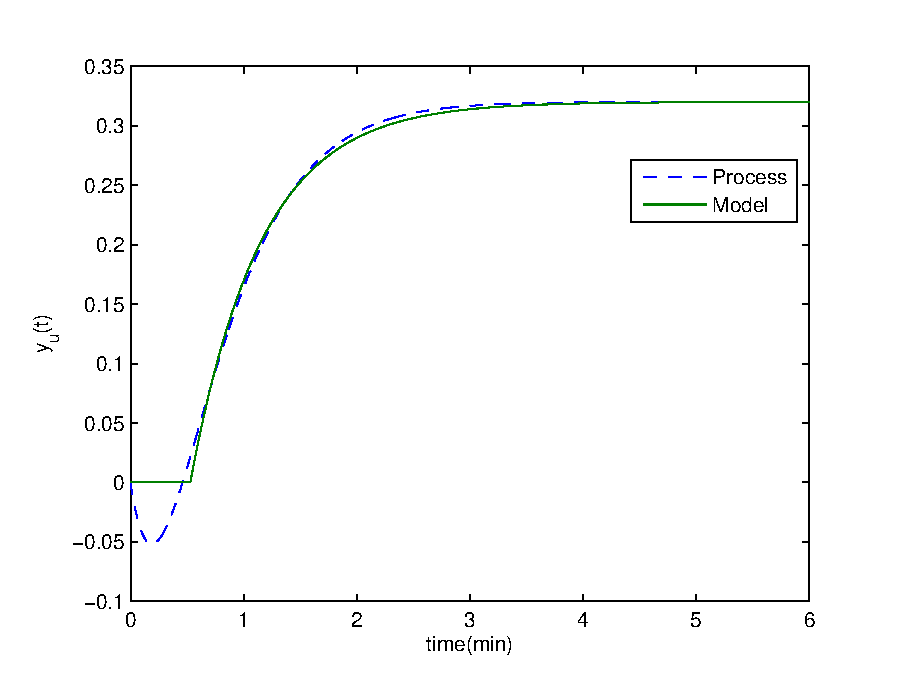
\includegraphics[width=0.7\linewidth]{FOPDT.eps}
       \caption{Example 2 - Reaction curve for process and FOPDT model} \label{process}
    \end{center}
\end{figure}

Using the identification method \cite{alfaro2006-1}, the
determined FOPDT model is

\be
    P_3(s) \approx \frac {0.3199 \me^{-0.5289 s}}{0.6238 s +1}
    \label{model_Pu}
\ee

From (\ref{model_Pu}), the application of the ISE tuning formulae
for optimal set-point and load-disturbance responses and also the
\emph{intermediate} $\overline{\gamma}_{\alpha}-autotuning$
provide the parameters for the PID controller that are shown in
Table \ref{PID_parameters3}.

\begin{table}[h!]
\begin{center}
\caption{Example 2 - PID Controller Parameters}
\begin{tabular}{c|ccc}
\hline \textbf{tuning}               &$K_p$ &$T_i$ &$T_d$\\ \hline
$set-point(sp)$                               &3.799  &0.707  &0.264 \\
$load-disturbance(ld)$                        &5.404  &0.494  &0.293 \\
\hline
$\overline{\gamma}_{\alpha=0.25}-autotuning$  &4.190  &0.609  &0.269 \\
$\overline{\gamma}_{\alpha=0.50}-autotuning$  &4.570  &0.577  &0.270 \\
$\overline{\gamma}_{\alpha=0.75}-autotuning$  &4.820  &0.551  &0.273 \\
\hline
\end{tabular}
\label{PID_parameters3}
\end{center}
\end{table}

Process outputs of the closed-loop system are shown in Fig.
\ref{y31}, first for a set-point step change of -10\%, follows by
a disturbance of +10\% and finally a new change in the set-point
of +5\%, all these situations using the three tuning modes
(set-point, load-disturbance and
$\overline{\gamma}_{\alpha}-autotuning$). Also, the control signal
($u(t)$) can be seen. It appears that, as expected, the control
signal is smoother for lower values of $\alpha$.

\begin{figure}[htb!]
    \begin{center}
        \includegraphics[width=0.7\linewidth]{y3outp1.eps}
       \caption{Example 2 - Process output for the non-linear control system operating in both servo and regulation modes} \label{y31}
    \end{center}
\end{figure}

A more comprehensive picture of the set-point change is shown in
Fig. \ref{y32}. In this case, it can be seen that, as expected,
the set-point tuning gives the better performance for servo
operation mode. Furthermore, the
$\overline{\gamma}_{\alpha}-autotuning$ provides a lower
degradation, respect to the optimal, than the load-disturbance
tuning.

\begin{figure}[htb!]
    \begin{center}
        \includegraphics[width=0.7\linewidth]{y3outp2.eps}
       \caption{Example 2 - Process output for the non-linear control system operating as servo} \label{y32}
    \end{center}
\end{figure}

The detail of load-disturbance attenuation is in Fig. \ref{y33}.
Similarly to the previous case, the load-disturbance tuning is the
one that gives better performance for regulation operation and the
performance degradation of the set-point tuning is greater than
the three cases for $\overline{\gamma}_{\alpha}-autotuning$.

\begin{figure}[htb!]
    \begin{center}
        \includegraphics[width=0.7\linewidth]{y3outp3.eps}
       \caption{Example 2 - Process output for the non-linear control system operating as regulator} \label{y33}
    \end{center}
\end{figure}

In general terms, it can be confirmed that the
$\overline{\gamma}_{\alpha}-autotuning$ gives a better performance
when the system operates in both servo and regulation modes. Also,
the control signal for the \emph{intermediate} tuning seems to be
\emph{smoother} than that provided by the optimal regulation
settings.

Table \ref{values_PDex3} shows the $\mathit{PD}$ and
$\mathit{WPD}$ indices and the improvement that can be achieve for
each case of the $\overline{\gamma}_{\alpha}-autotuning$.\\

\begin{table}[htb!]
\begin{center}
\caption{Example 2 - $\mathit{PD}$ and $\mathit{WPD}$ values for
the non-linear CSTR system and the improvement obtained with
$\overline{\gamma}_{\alpha}-autotuning$}
\begin{tabular}{c|cc|ccc}
\hline \textbf{tuning}       &$PD_{sp}$  &$PD_{ld}$ &$WPD_{\alpha=0.25}$ &$WPD_{\alpha=0.50}$ &$WPD_{\alpha=0.75}$\\
\hline
$set-point(sp)$                               &-          &0.3284 &0.0821 &0.1642 &0.2463\\
$load-disturbance(ld)$                        &0.5316     &-      &0.3987 &0.2658 &0.1329\\
$\overline{\gamma}_{\alpha=0.25}-autotuning$  &0.0192     &0.1398 &0.0493 &- &-\\
$\overline{\gamma}_{\alpha=0.50}-autotuning$  &0.0706     &0.0470 &- &0.0588 &-\\
$\overline{\gamma}_{\alpha=0.75}-autotuning$  &0.1334     &0.0038 &- &- &0.0362\\
\hline \hline
improvement in \% of                          &            &            & & &\\
\hline
$\overline{\gamma}_{\alpha=0.25}-autotuning$  &96.39\%(ld) &57.73\%(sp) &39.95\%(sp) &- &-\\
                                              &            &            &87.63\%(ld) &- &-\\
$\overline{\gamma}_{\alpha=0.50}-autotuning$  &86.72\%(ld) &85.99\%(sp) &- &64.19\%(sp) &-\\
                                              &            &            &- &77.88\%(ld) &-\\
$\overline{\gamma}_{\alpha=0.75}-autotuning$  &74.91\%(ld) &99.15\%(sp) &- &- &85.30\%(sp)\\
                                              &            &            &- &- &72.76\%(ld)\\
(respect to)                                  &            &            & & &\\
\hline
\end{tabular}
\label{values_PDex3}
\end{center}
\end{table}
